\epi{``I'm always delighted by the light touch and stillness of
early programming languages.  Not much text; a lot gets
done. Old programs read like quiet conversations
between a well-spoken research worker and a well-
studied mechanical colleague, not as a debate with a
compiler.  Who'd have guessed sophistication bought
such noise?''}{\textsc{RICHARD P. GABRIEL}}

\noindent{}Functions are the basic building blocks of Go programs; all interesting
stuff happens in them. A function is declared as follows:
\begin{lstlisting}[caption=A function declaration,label=src:function definition]
|\begin{tikzpicture}[overlay]
\ubrace{0.6,-1.5}{0.0,-1.5}{The keyword \key{func} is used to declare a function;}
%
\ubrace{2.2,-1.5}{0.8,-1.5}{A function can be defined to work on a specific type, a %
more common name for such a function is \index{method}{method}. This part is %
called a \first{\emph{receiver}}{receiver} and it is optional. See %
chapter \ref{chap:interfaces};}
%
\ubrace{3.4,-1.5}{2.4,-1.5}{\emph{funcname} is the name of your function;}
%
\ubrace{4.5,-1.5}{3.6,-1.5}{The variable \var{q} of type \type{int} is %
the input parameter. The parameters are passed %
\first{\emph{pass-by-value}}{pass-by-value} meaning they are copied. %
But be aware that reference types (slices, channels, maps and interfaces) are %
\first{\emph{pass-by-reference}}{pass-by-reference} even though you %
do not see the pointers directly in the code;}
%
\ubrace{6.0,-1.5}{4.9,-1.5}{%
The variables \var{r} and \var{s} are the %
\index{named return parameters}{named return parameters} for this function. %
Note that functions in Go can have multiple return values. See section %
"\titleref{sec:multiple return}" on page \pageref{sec:multiple return} %
for more information. If you want the return %
parameters not to be named you only give the types: %
\lstinline{(int,int)}. If you have only one value to return you may omit %
the parentheses. If your function is a subroutine and does not have %
anything to return you may omit this entirely;}
%
\ubrace{8.2,-1.5}{6.3,-1.5}{This is the function's body, note that %
\func{return} is a statement so the braces around the parameter(s) are %
optional.}
\end{tikzpicture}|
type mytype int	|\coderemark{New type, see chapter \ref{chap:beyond}}|

func (p mytype) funcname(q int) (r,s int) { return 0,0 }
||
\end{lstlisting}

\showremarks
Here are two examples. On the left is a function without a return value,
while on the right is a simple function that returns its input.

\begin{minipage}{.5\textwidth}
\begin{lstlisting}
func subroutine(in int) {
    return
}
\end{lstlisting}
\end{minipage}
\begin{minipage}{.5\textwidth}
\begin{lstlisting}
func identity(in int) int {
    return in
}
\end{lstlisting}
\end{minipage}

Functions can be declared in any order you wish. The compiler scans the
entire file before execution, so function prototyping is a thing of the
past in Go. Go disallows nested functions, but you can work around this with
anonymous functions. See section ``\titleref{sec:functions as values}'' on page
\pageref{sec:functions as values} in this chapter.

Recursive functions work just as in other languages:
\begin{lstlisting}[caption=Recursive function]
func rec(i int) {
   if i == 10 {
        return
   }
   rec(i+1)
   fmt.Printf("%d ", i)
}
\end{lstlisting}
This prints: \texttt{9 8 7 6 5 4 3 2 1 0}.
%%\newpage %% TODO don't want a newpage here actually
\section{Scope}
Variables declared outside any functions are \first{global}{scope!local} in Go, those
defined in functions are \first{local}{scope!local} to those functions. If names overlap --- a
local variable is declared with the same name as a global one --- the
local variable hides the global one when the current function is
executed.

\begin{minipage}{.5\textwidth}
\begin{lstlisting}[linewidth=.5\textwidth,caption=Local scope]
|\begin{tikzpicture}[overlay]
\draw [->,thick] (3.1,-5.00) arc (-60:90:2.00cm);
\draw [->,thick] (3.1,-7.00) arc (-60:90:0.20cm);
\end{tikzpicture}|
package main

var a = 6

func main() {
        p()
        q()
        p()
}

func p() {
        println(a)
}

func q() {
        a := 5
        println(a)
}
\end{lstlisting}

\hfill
\vfill
\end{minipage}
\hfill
\begin{minipage}{.5\textwidth}
\begin{lstlisting}[caption=Global scope,label=src:scope2]
|\begin{tikzpicture}[overlay]
\draw [->,thick] (2.8,-5.00) arc (-60:90:2.00cm);
\draw [->,thick] (3.4,-7.00) arc (-60:90:3.15cm);
\end{tikzpicture}|
package main

var a = 6

func main() {
    p()
    q()
    p()
}

func p() {
    println(a)
}

func q() {
    a = 5|\coderemark{Assignment}|
    println(a)
}
\end{lstlisting}

\hfill
\vfill
\end{minipage}

In listing \ref{src:scope1} we introduce a local variable \var{a}
in the function \func{q()}.
The local \var{a} is only visible in \func{q()}. This is
why the code will print: \texttt{656}.
In listing \ref{src:scope2} no new variables are introduced, there
is only a global \var{a}.
Assigning a new value to \var{a} will be globally visible. This code will
print: \texttt{655}

In the following example we call \func{g()} from \func{f()}:

\lstinputlisting[caption=Scope when calling functions from functions]{src/scope3.go}

The output will be: \texttt{565}. A \emph{local} variable is \emph{only}
valid when we are executing the function in which it is defined. 
%%Finally, one can create a \first{"function literal"}{function literal} in which you essentially 
%%define a function inside another
%%function, i.e. a \first{nested function}{nested function}. 
%%The following figure should clarify why it prints: \texttt{565757}. 
%%\begin{lstlisting}[caption=Scope and function literals,label=src:scope3,float]
|\begin{tikzpicture}[overlay]
\draw [->,thick] (2.8,-4.10) arc (-60:90:0.20cm);
\draw [->,thick] (2.8,-2.00) arc (-60:90:0.20cm);
\draw [->,thick] (2.4,-1.60) arc (-60:90:0.50cm);
%
\draw [->,thick] (4.4,-8.75) arc (-60:80:4.30cm);
% function f()
\draw [->,thick] (4.4,-5.85) arc (-60:90:0.30cm);
\draw [->,thick] (4.4,-5.25) arc (-60:90:0.90cm);
%
\draw [->,thick] (3.2,-7.45) arc (-60:65:2.00cm);
\end{tikzpicture}|
package main
var a int
func main() {
        a = 5
        println(a)
        f()
}
func f() {
        a := 6
        println(a)
        g()
        x := func() {
                a = 7
                println(a)
        }
        x()
        g()
        println(a)
}
func g() {
        println(a)
}
\end{lstlisting}


\section{Multiple return values}
\label{sec:multiple return}
One of Go's unusual (for compiled languages) features is that functions and methods can return multiple
values (Python and Perl can do this too). This can be used to improve on a couple of 
clumsy idioms in C programs:
in-band error returns (such as -1 for \texttt{EOF}) and modifying an argument.
In Go, \lstinline{Write} returns a count and an
error: ``Yes, you wrote some bytes but not all of them because you filled the
device''. The signature of \lstinline{*File.Write} in package
\package{os} is:
\begin{lstlisting}
func (file *File) Write(b []byte) (n int, err error)
\end{lstlisting}
and as the documentation says, it returns the number of bytes written and a
non-\lstinline{nil} \var{error} when \lstinline{n != len(b)}. This is a common
style in Go.

A similar approach obviates the need to pass a pointer to a return value to
simulate a reference parameter. Here's a simple-minded function to grab a
number from a position in a byte array, returning the number and the next
position.
\begin{lstlisting}
func nextInt(b []byte, i int) (int, int) {
    x := 0
    // Naively assume everything is a number
    for ; i < len(b); i++ {
        x = x*10 + int(b[i]) - '0'
    }
    return x, i
}
\end{lstlisting}
You could use it to scan the numbers in an input array \var{a} like this:
\begin{lstlisting}
a := []byte{'1', '2', '3', '4'}
var x int
for i := 0; i < len(a); {	|\coderemark{No \texttt{i++}}|
    x, i = nextInt(a, i)
    println(x)
}
\end{lstlisting}
In the absence of tuples as a native type, multiple return values are the next
best thing. You can return precisely what you want without
overloading the domain space with special values to signal errors.

\section{Named result parameters}
\label{sec:named result parameters}
The return or result parameters of a Go function can be given names and used
as regular variables, just like the incoming parameters. When named, they are
initialized to the zero values for their types when the function begins; if the
function executes a \key{return} statement with no arguments, the current values of
the result parameters are used as the returned values. Using these
features enables you (again) to do more with less code \footnote{This is
a motto of Go; ``Do \emph{more} with \emph{less} code''}.

The names are not mandatory but they can make code shorter and clearer:
\emph{they are documentation}. 
If we name the results of \lstinline{nextInt} it becomes obvious which
returned \type{int} is which.

\begin{lstlisting}
func nextInt(b []byte, pos int) (value, nextPos int) { /* ... */ }
\end{lstlisting}
Because named results are initialized and tied to an unadorned
\key{return},
they can simplify as well as clarify. Here's a version of
\lstinline{io.ReadFull} that uses them well:

\begin{lstlisting}
func ReadFull(r Reader, buf []byte) (n int, err error) {
    for len(buf) > 0 && err == nil {
        var nr int
        nr, err = r.Read(buf)
        n += nr
        buf = buf[nr:len(buf)]
    }
    return
}
\end{lstlisting}

\section{Deferred code}
\label{sec:deferred code}
Suppose you have a function in which you open a file and perform various
writes and reads on it. In such a function there are often spots where
you want to return early. If you do that, you will need to close the file
descriptor you are working on. This often leads to the following code:
\begin{lstlisting}[caption=Without defer]
func ReadWrite() bool {
    file.Open("file")
    // Do your thing
    if failureX {
	file.Close() |\coderemark{}|
	return false
    }

    if failureY {
	file.Close() |\coderemark{}|
	return false
    }
    file.Close() |\coderemark{}|
    return true
}
\end{lstlisting}
A lot of code is repeated here. To overcome this Go has the
\first{\key{defer}}{keyword!defer} statement. After
\key{defer} you specify a function which is called just \emph{before}
the current function exits.

The code above could be rewritten as follows. This makes the 
function more readable, shorter and puts the \func{Close} right next 
to the \func{Open}.
\begin{lstlisting}[caption=With defer]
func ReadWrite() bool {
    file.Open("file")
    defer file.Close()	|\coderemark{\func{file.Close()} is added to the defer list}|
    // Do your thing
    if failureX {
	return false    |\coderemark{\func{Close()} is now done automatically}|
    }
    if failureY {
	return false    |\coderemark{And here too}|
    }
    return true
}
\end{lstlisting}
You can put multiple functions on the ``deferred list''\index{deferred list}, like this
example from \cite{effective_go}:
\begin{lstlisting}
for i := 0; i < 5; i++ { 
    defer fmt.Printf("%d ", i) 
} 
\end{lstlisting}
Deferred functions are executed in LIFO order, so the above code
prints: \lstinline{4 3 2 1 0}. 

With \func{defer} you can even change return values, provided that
you are using named result parameters and a function
literal\index{function!literal}\footnote{A function literal
is sometimes called a \index{closure} closure.}, i.e:
\begin{lstlisting}[caption=Function literal]
defer func() {
	/* ... */
}()		 |\coderemark{() is needed here}|
\end{lstlisting}
Or this example which makes it easier to understand why and where
you need the braces:
\begin{lstlisting}[caption=Function literal with parameters]
defer func(x int) {
	/* ... */
}(5)		 |\coderemark{Give the input variable \var{x} the value 5}|
\end{lstlisting}
In this (unnamed) function you can access any named return
parameter:
\begin{lstlisting}[caption=Access return values within defer]
func f() (ret int) {    |\coderemark{\var{ret} is initialized with zero}|
	defer func() {
		ret++	|\coderemark{Increment \var{ret} with 1}|
	}()
	return 0	|\coderemark{1 \emph{not} 0 will be returned!}|
}
\end{lstlisting}

\section{Variadic parameters}
Functions that take variadic parameters are functions that have a
variable number of parameters. To do this, you first
need to declare your function to take variadic arguments:
\begin{lstlisting}
func myfunc(arg ...int) {}
\end{lstlisting}
The \lstinline{arg ...int} instructs Go to see this as a function that
takes a variable number of arguments. Note that these arguments all
have the type \type{int}. Inside your function's body the variable
\var{arg} is a slice of ints:
\begin{lstlisting}
for _, n := range arg {
    fmt.Printf("And the number is: %d\n", n)
}
\end{lstlisting}
If you don't specify the type of the variadic argument it defaults to the
empty interface \var{interface\{\}} (see chapter
\ref{chap:interfaces}).
Suppose we have another variadic function called \func{myfunc2}, the 
following example shows how to pass variadic arguments to it:
\begin{lstlisting}
func myfunc(arg ...int) {
    myfunc2(arg...)  |\coderemark{Pass it as-is}|
    myfunc2(arg[:2]...)  |\coderemark{Slice it}|
}
\end{lstlisting}

\section{Functions as values}
\label{sec:functions as values}
\index{function!as values}
\index{function!literals}
As with almost everything in Go, functions are also \emph{just} values.
They can be assigned to variables as follows:
\lstinputlisting[label=src:anonfunc,caption=Anonymous function,linerange={3,}]{src/anon-func.go}
If we use \lstinline{fmt.Printf("%T\n", a)} to print the type of
\var{a}, it prints \func{func()}.

Functions--as--values may also be used in other places, like in maps.
Here we convert from integers to functions:
\begin{lstlisting}[caption=Functions as values in maps]
var xs = map[int]func() int{
    1: func() int { return 10 },
    2: func() int { return 20 },
    3: func() int { return 30 }, |\coderemark{Mandatory ,}|
    /* ... */
}
\end{lstlisting}
Or you can write a function that takes a function as its parameter, for
example a \func{Map} function that works on \type{int} slices. This is
left as an exercise for the reader (see exercise Q\ref{ex:map function}
on page \pageref{ex:map function}).

\section{Callbacks}
\label{sec:callbacks}
With functions as values they are easy to pass to functions, from where
they can be used as callbacks. First define a function that
does ``something'' with an integer value:
\begin{lstlisting}
func printit(x int) {       |\coderemark{Function returns nothing}|
    fmt.Printf("%v\n", x)    |\coderemark{Just print it}|
}
\end{lstlisting}
The signature of this function is: \lstinline{func printit(int)}, or
without the function name: \mbox{\lstinline{func(int)}}. To create a new function
that uses this one as a callback we need to use this signature:
\begin{lstlisting}
func callback(y int, f func(int)) { |\coderemark{\func{f} will hold the function}|
    f(y)    |\coderemark{Call the callback \func{f} with \var{y}}|
}
\end{lstlisting}

\section{Panic and recovering}
\label{sec:panic}
Go does not have an exception mechanism, like that in Java for instance: you can not throw exceptions.
Instead it uses a panic-and-recover mechanism. It is worth remembering that you should use this as
a last resort, your code will not look, or be, better if it is littered with panics. It's a powerful tool:
use it wisely. So, how do you use it?

The following description was taken from \cite{go_blog_panic}:
\begin{description}
\item[Panic]{is a built-in function that stops the ordinary flow of control and begins panicking. When the function 
\func{F} calls \key{panic},
execution of \func{F} stops, any deferred functions in \func{F} are executed normally, and 
then \func{F} returns to its caller. To the caller, \func{F} then
behaves like a call to \key{panic}. The process continues up the stack until all functions in the current 
goroutine have returned, at which point the program crashes. 

Panics can be initiated by invoking \func{panic} directly. They can also be caused by \emph{runtime errors}, such
as out-of-bounds array accesses.}

\item[Recover]{is a built-in function that regains control of a panicking goroutine. Recover is \emph{only} useful inside 
\emph{deferred} functions.

During normal execution, a call to \func{recover} will return \type{nil} and have no other effect. 
If the current goroutine is panicking, a call
to \func{recover} will capture the value given to \func{panic} and resume normal execution.}
\end{description}

This function checks if the function it gets as argument will panic when it is
executed\footnote{Copied from a presentation of Eleanor McHugh.}:
\begin{lstlisting}
func throwsPanic(f func()) (b bool) { |\longremark{We define a new function \func{throwsPanic} that takes %
a fuction as an argument, see ``\titleref{sec:functions as values}''. It returns true when this function %
will panic, otherwise false;}|
    defer func() { |\longremark{We define a \func{defer} function that utilizes \func{recover}, \emph{if} the %
current goroutine panics, this defer function will notice that. If \func{recover()} returns non-\var{nil} we set \var{b} %
to true;}|
        if x := recover(); x != nil {
            b = true
        }
    }()
    f() |\longremark{Execute the function we received as the argument;}|
    return |\longremark{Return the value of \var{b}. Because \var{b} is a named return parameter (page %
\pageref{sec:named result parameters}), we don't specify \var{b}.}|
}
\end{lstlisting}
\showremarks


\section{Exercises}
\begin{Exercise}[title={平均值},difficulty=4]
\label{ex:average}
\Question\label{ex:average q1} 编写一个函数用于计算一个~\type{float64} 类型的~slice 的平均值。
\end{Exercise}

\begin{Answer}
\Question 下面的函数计算平均值。
\lstinputlisting[caption=Go 中的平均值函数,linerange={3,14}]{ex-functions/src/ave.go}
\showremarks
\end{Answer}


\begin{Exercise}[title={Integer ordering},difficulty=3]
\label{ex:ordering function}
\Question Write a function that returns it parameters in the right,
numerical (ascending) order:\newline 
\lstinline{f(7,2)} $\rightarrow$ \lstinline{2,7}\newline
\lstinline{f(2,7)} $\rightarrow$ \lstinline{2,7}\newline
\end{Exercise}

\begin{Answer}
\todo{Write the answer (MG).}
\Question

\end{Answer}




\begin{Exercise}[title={Scope},difficulty=4]
\label{ex:scope}
\Question\label{ex:scope q1} What is wrong with the following program?

\begin{lstlisting}[numbers=right]
package main

import "fmt"
                                                                                                   
func main() {
        for i := 0; i < 10; i++ {
                fmt.Printf("%v\n", i)
        }
	fmt.Printf("%v\n", i)
}
\end{lstlisting}

\end{Exercise}

\begin{Answer}
\Question
The program does not even compile, because \var{i} on line 9 is
not defined: \var{i} is only defined within the \key{for}-loop. To fix
this the function \func{main()} should become:
\begin{lstlisting}[numbers=none]
func main() {
        var i int
        for i = 0; i < 10; i++ {
                fmt.Printf("%v\n", i)
        }
	fmt.Printf("%v\n", i)
}
\end{lstlisting}
Now \var{i} is defined outside the \key{for}-loop and still visible
afterwards. This code will print the numbers 0 through 10.
\end{Answer}


\begin{Exercise}[title={Stack},difficulty=5]
\label{ex:stack}
\Question \label{ex:stack q1} Create a simple stack which can hold a
fixed amount of \key{int}s. Is does not have to grow beyond this limit.
Define both a \func{push} and \func{pop} function.

\begin{wrapfigure}{l}{30mm}
\begin{center}
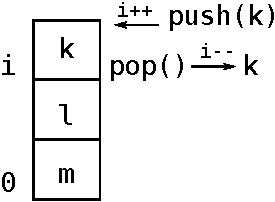
\includegraphics[scale=0.50]{fig/stack.pdf}
\end{center}
\end{wrapfigure}

\Question \label{ex:stack q2} Bonus. Write a \func{String} method which 
converts the stack to a string. This way you can print the stack using:
\lstinline{fmt.Printf("My stack %v\n", stack)}. This may aid in
debugging.
\end{Exercise}

\begin{Answer}

\Question 

\Question 

\end{Answer}


\begin{Exercise}[title={Var args},difficulty=5]
\label{ex:varargs}
\Question\label{ex:varargs q1}
Write a function that takes a variable numbers of \type{int}s and prints
each integer on a seperate line
\end{Exercise}

\draft{BETER}
\begin{Answer}
\Question
For this we need the \lstinline{...}-syntax so signal we have a
function that takes an arbitrary number of arguments.

\lstinputlisting[label=src:varargs,caption=A function with variable number of arguments]{ex-functions/src/var-arg.go}

\end{Answer}


\begin{Exercise}[title={斐波那契},difficulty=5]
\label{ex:fibonaci}
\Question\label{ex:fibonaci q1}
斐波那契数列以:$1, 1, 2, 3, 5, 8, 13, \ldots$ 开始。
或者用数学形式表达:$ x_1 = 1; x_2 = 1; x_n = x_{n-1} +
x_{n-2}\quad\forall n > 2 $。

编写一个函数,接受 \type{int} 值,并给出这个值得到的斐波那契数列。

\end{Exercise}

\begin{Answer}
\Question
下面的程序会计算出斐波那契数列。
\lstinputlisting[label=src:fib,caption=Fibonacci function in Go]{ex-functions/src/fib.go}

\showremarks
\end{Answer}


\begin{Exercise}[title={Map function},difficulty=4]
\label{ex:map function}
A \func{map()}-function is a function that takes
a function and a list. The function is applied to 
each member in the list and a new list containing
these calculated values is returned.
Thus: 
$$ map(f(), (a_1,a_2,\ldots,a_{n-1},a_n)) =  (f(a_1), f(a_2),\ldots,f(a_{n-1}), f(a_n)) $$
\Question \label{ex:map function q1} Write a simple
\func{map()}-function in Go. It is sufficient
for this function only to work for ints.
\Question \label{ex:map function q2} Expand your code to also work on a list of strings.

\end{Exercise}

\begin{Answer}

\Question 
\begin{lstlisting}[caption=A \func{Map} function]
func Map(f func(int) int, l []int) []int {
        j := make([]int, len(l))
        for k, v := range l {
                j[k] = f(v)
        }
        return j
}

func main() {
        m := []int{1, 3, 4}
        f := func(i int) int {
                return i * i
        }
        fmt.Printf("%v", (Map(f, m)))
}
\end{lstlisting}

\Question Answer to question but now with strings
\end{Answer}




\begin{Exercise}[title={Minimum and maximum},difficulty=0]
\label{ex:minmax}
\Question\label{ex:minmax q1} Write a function that finds the
maximum value in an \type{int} slice (\type{[]int}).

\Question\label{ex:minmax q2} Write a function that finds the
minimum value in an \type{int} slice (\type{[]int}).

\end{Exercise}

\begin{Answer}
\Question This function returns the largest int in the slice \var{l}:
\begin{lstlisting}
func max(l []int) (max int) {   |\longremark{We use a named return parameter;}|
        max = l[0]      
        for _, v := range l {   |\longremark{Loop over \var{l}. The index of the element is %
not important;}|
                if v > max {    |\longremark{If we find a new maximum, remember it;}|
                        max = v 
                }   
        }   
        return  |\longremark{A ``lone'' return, the current value of \var{max} is now returned.}|
}
\end{lstlisting}
\showremarks

\Question This function returns the smallest int in the slice \var{l}. It is almost identical to \func{max}:
\begin{lstlisting}
func min(l []int) (min int) {
        min = l[0]
        for _, v := range l { 
                if v < min {
                        min = v 
                }   
        }   
        return
}
\end{lstlisting}
The interested reader may combine \func{max} and \func{min} into one function with a selector
that lets you choose between the minimum or the maximum, or one that returns both values.
\end{Answer}


\begin{Exercise}[title={Bubble sort},difficulty=1]
\label{ex:bubble}
\Question\label{ex:bubble q1} Write a function that performs 
Bubble sort on slice of ints. From \cite{bubblesort}:
\begin{quote}
It works by repeatedly stepping through the list to be sorted, comparing each
pair of adjacent items and swapping them if they are in the wrong order. The
pass through the list is repeated until no swaps are needed, which indicates
that the list is sorted. The algorithm gets its name from the way smaller
elements ``bubble'' to the top of the list. 
\end{quote}

\cite{bubblesort} also gives an example in pseudo code:
\begin{lstlisting}[language=pascal]
procedure bubbleSort( A : list of sortable items )
  do
    swapped = false
    for each i in 1 to length(A) - 1 inclusive do:
      if A[i-1] > A[i] then
        swap( A[i-1], A[i] )
        swapped = true
      end if
    end for
  while swapped
end procedure
\end{lstlisting}
\end{Exercise}

\begin{Answer}
\Question 
The Bubble sort isn't terribly efficient, for $n$ elements it scales
$O(n^2)$. See QuickSort \cite{quicksort} for a better sorting algorithm.

But Bubble sort is easy to implement, the following is an example.
\lstinputlisting[caption=Bubble sort,linerange=4-19]{ex-functions/src/bubblesort.go}

Because a slice is a reference type the \func{bubblesort} function works and
does not need to return a sorted slice.
\end{Answer}


\begin{Exercise}[title={Functions that return functions},difficulty=1]
\label{ex:function}
\Question\label{ex:function q1} Write a function that returns a function
that performs a $+2$ on integers. Name the function \func{plusTwo}.
You should then be able do the following:
\begin{lstlisting}
p := plusTwo()
fmt.Printf("%v\n", p(2))
\end{lstlisting}
Which should print 4.
See section \titleref{sec:callbacks} on page \pageref{sec:callbacks} for information
about this topic.

\Question\label{ex:function q2} Generalize the function from \ref{ex:function q1},
and create a \func{plusX(x)} which returns a functions that add \var{x} to an
integer.
\end{Exercise}

\begin{Answer}
\Question
\begin{lstlisting}
func main() {
        p2 := plusTwo()
        fmt.Printf("%v\n",p2(2))
}

func plusTwo() func(int) int { |\longremark{Define a new function that returns a function. %
See how you you can just write down what you mean;}|
        return func(x int) int { return x + 2 } |\longremark{Function literals at work, %
we define the +2--function right there in the return statement.}|
}
\end{lstlisting}
\showremarks

\Question
Here we use a closure:
\begin{lstlisting}
func plusX(x int) func(int) int { |\longremark{Again define a function that returns %
a function;}|
        return func(y int) int { return x + y } |\longremark{Use the \emph{local} variable %
\var{x} in the function literal.}|
}
\end{lstlisting}
\showremarks
\end{Answer}


\cleardoublepage
\section{Answers}
\shipoutAnswer
